
%%% Local Variables:
%%% mode: latex
%%% TeX-master: "../Tesis"
%%% End:
\chapter{Particle Accelerators}
\label{c:accel} % For referencing the chapter elsewhere, use \ref{} 
\lhead{Chapter~\ref{c:accel}.
  Accelerators} % This is for the header on each page - perhaps a shortened title
Particle accelerators are machines whose name is self explanatory. They were
originally developed for nuclear physics. Although we could argue that a
cathodic tube is an accelerator itself, we count as the first accelerator one
that was designed, after Rutherford challenged the scientific community in 1927
to accelerate charged particles to energies higher than natural
$\alpha$-decays\cite{Steere2005timeline}, which have a typical energy of
\SI{5}{MeV}.
% Cockcroft-Walton
This accelerator was the Cockcroft-Walton multiplier, which was used to produce the first ever reported nuclear fission. The original setup
is shown in Fig.~\ref{fig:cock}. It consisted of an AC power source charging a
ladder of capacitors by means of diodes, generating a large voltage
output\cite{Cockcroft619}. Following the relation between the electric field
($\vec{E}$) and the scalar potential ($V$): $\vec{E}=-\nabla{V}$ and equating
Newton's second law of motion ($\vec{F}=m\vec{a}$) to the Lorentz force
($\vec{F}=q(\vec{E}+\vec{v}\times\vec{B})$) we infer that the acceleration in an
electrostatic accelerator such as the Cockcroft-Walton is:
$\vec{a}=-\frac{q}{m}\nabla{}V$. Ever since, accelerators have not stopped
evolving. Scientists kept building larger and larger accelerators until they hit
a limit with electrostatic fields due to voltage breakdown\cite{EASTHAM1984101}.
% I poupusefully missed the van der graff generator

\begin{figure}
\centering
 \begin{minipage}{\textwidth}
 \centering
  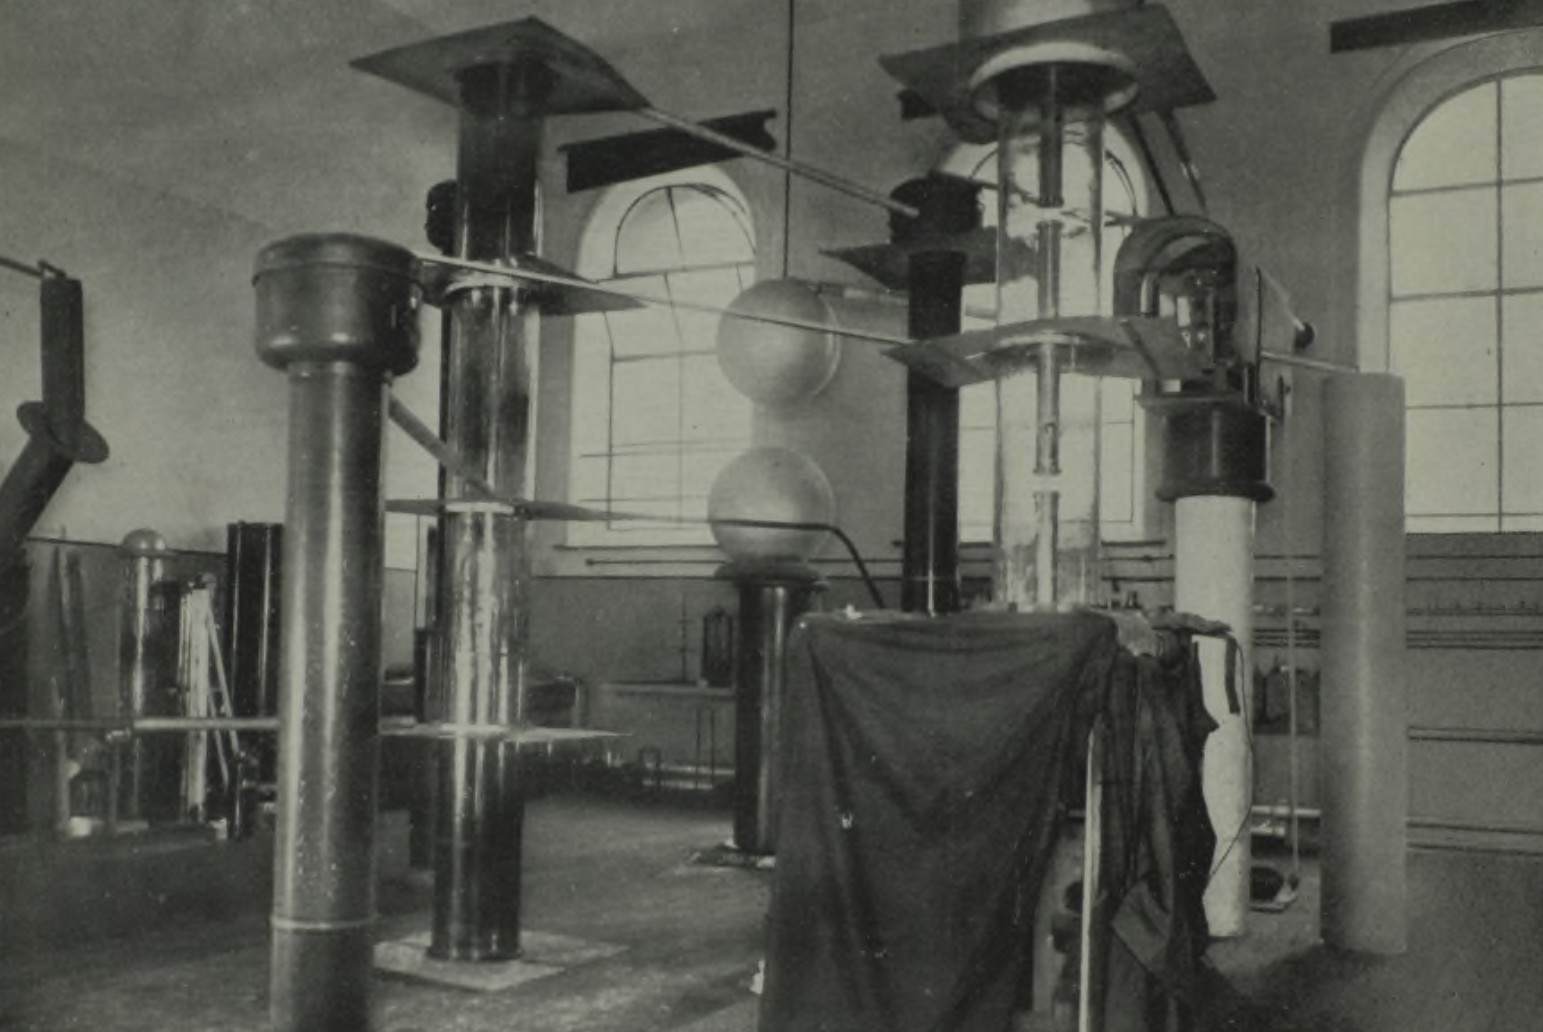
\includegraphics[width=3.5in]{Pictures/cockroft.jpg}
  \caption{\label{fig:cock}
   	Cockcroft-Walton accelerator original setting.}
   	\footnotesize{Picture taken from \citep{Cockcroft619}}
   \end{minipage}
\end{figure}
% RF Accelera6tors
% LINACS
A new technique for accelerating charges emerged. Already in 1924 Gustav Ising
had proposed using drift tubes to shield the charged particle from a pulsed
voltage\cite{Ising}, and in 1928 Rolf Wider\"oe suggested using a radiofrequency
(RF) system \cite{Wideroe1928}. To prove this principle Wider\"oe built the
first linear accelerator or linac, and RF acceleration was born.
%Cyclotron
Using the RF acceleration principle and one of Wider\"oe's ideas, Ernest
Lawrence set electrons in a curved path by applying a perpendicular magnetic
field so that the electrons would pass several times through and accelerating
gap. Figure \ref{fig:cyclo} shows Lawrence drawings in his 1934 patent and in
Fig. \ref{fig:lawrence} we see Lawrence standing next to his \SI{1.5}{m}
diameter cyclotron in the University of California at Berkeley.
\begin{figure}
 \centering
  \begin{minipage}{\textwidth}
  \centering
   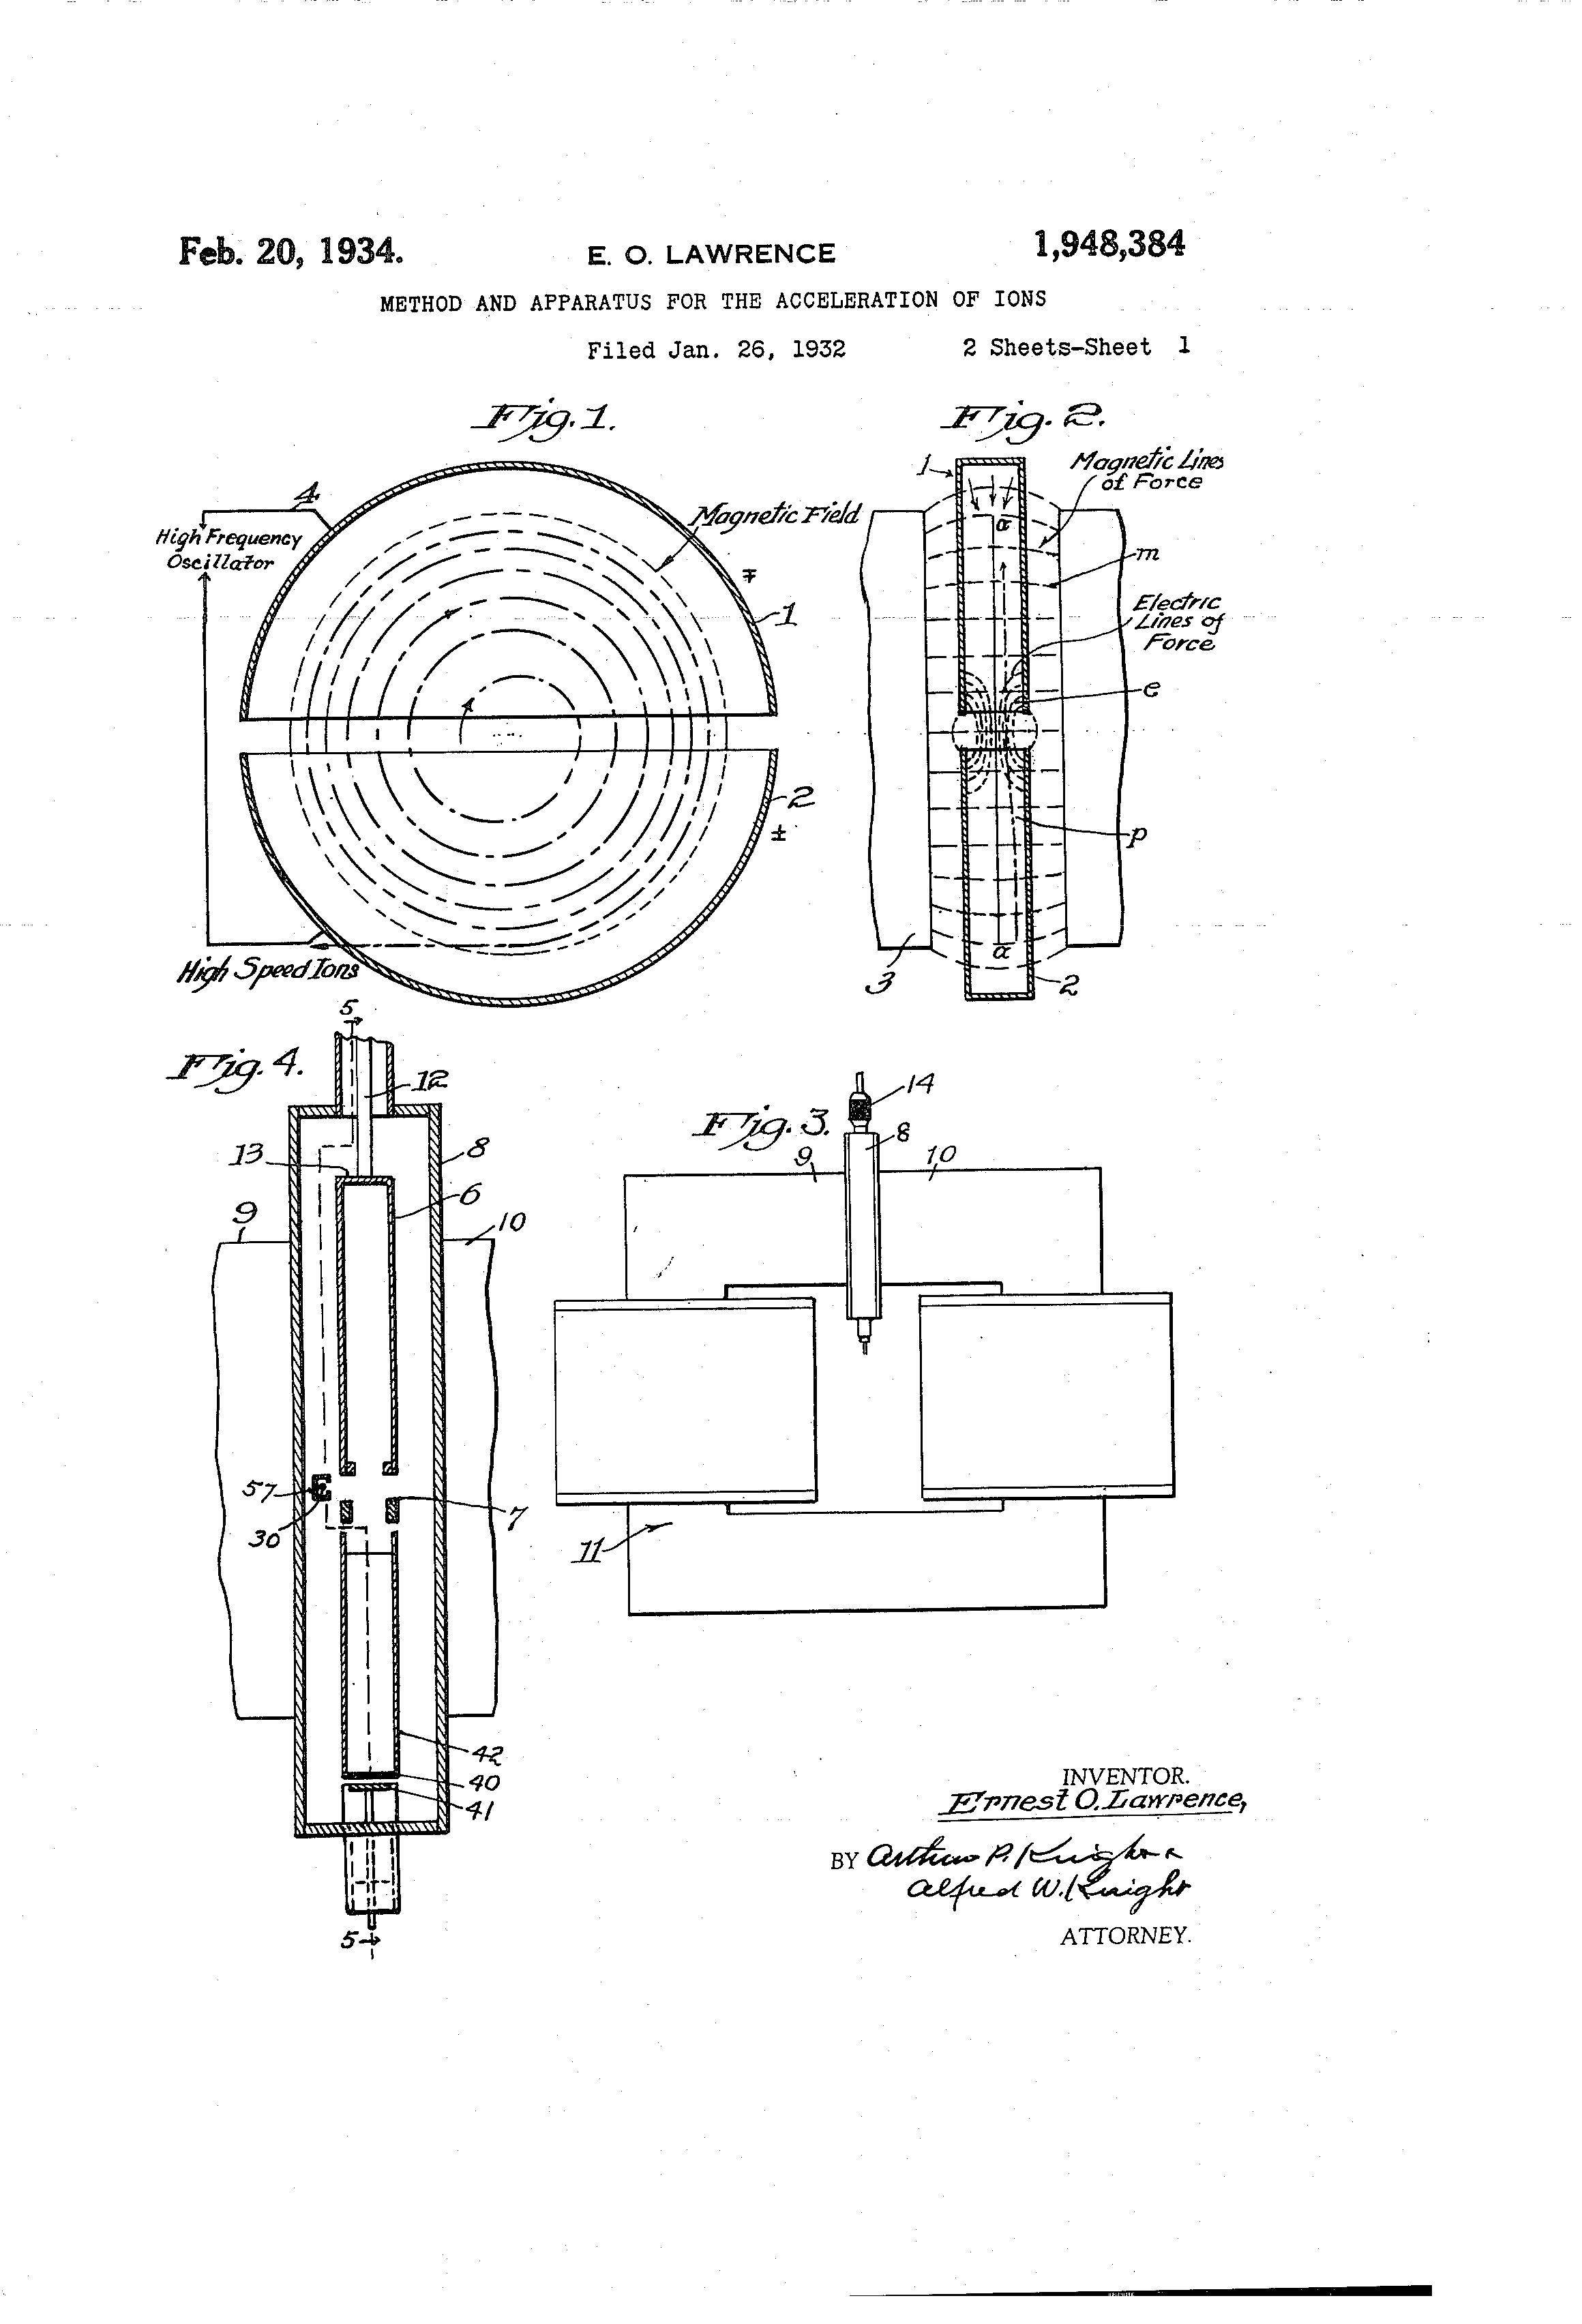
\includegraphics[width=.49\textwidth]{Pictures/cyclo1.png}
   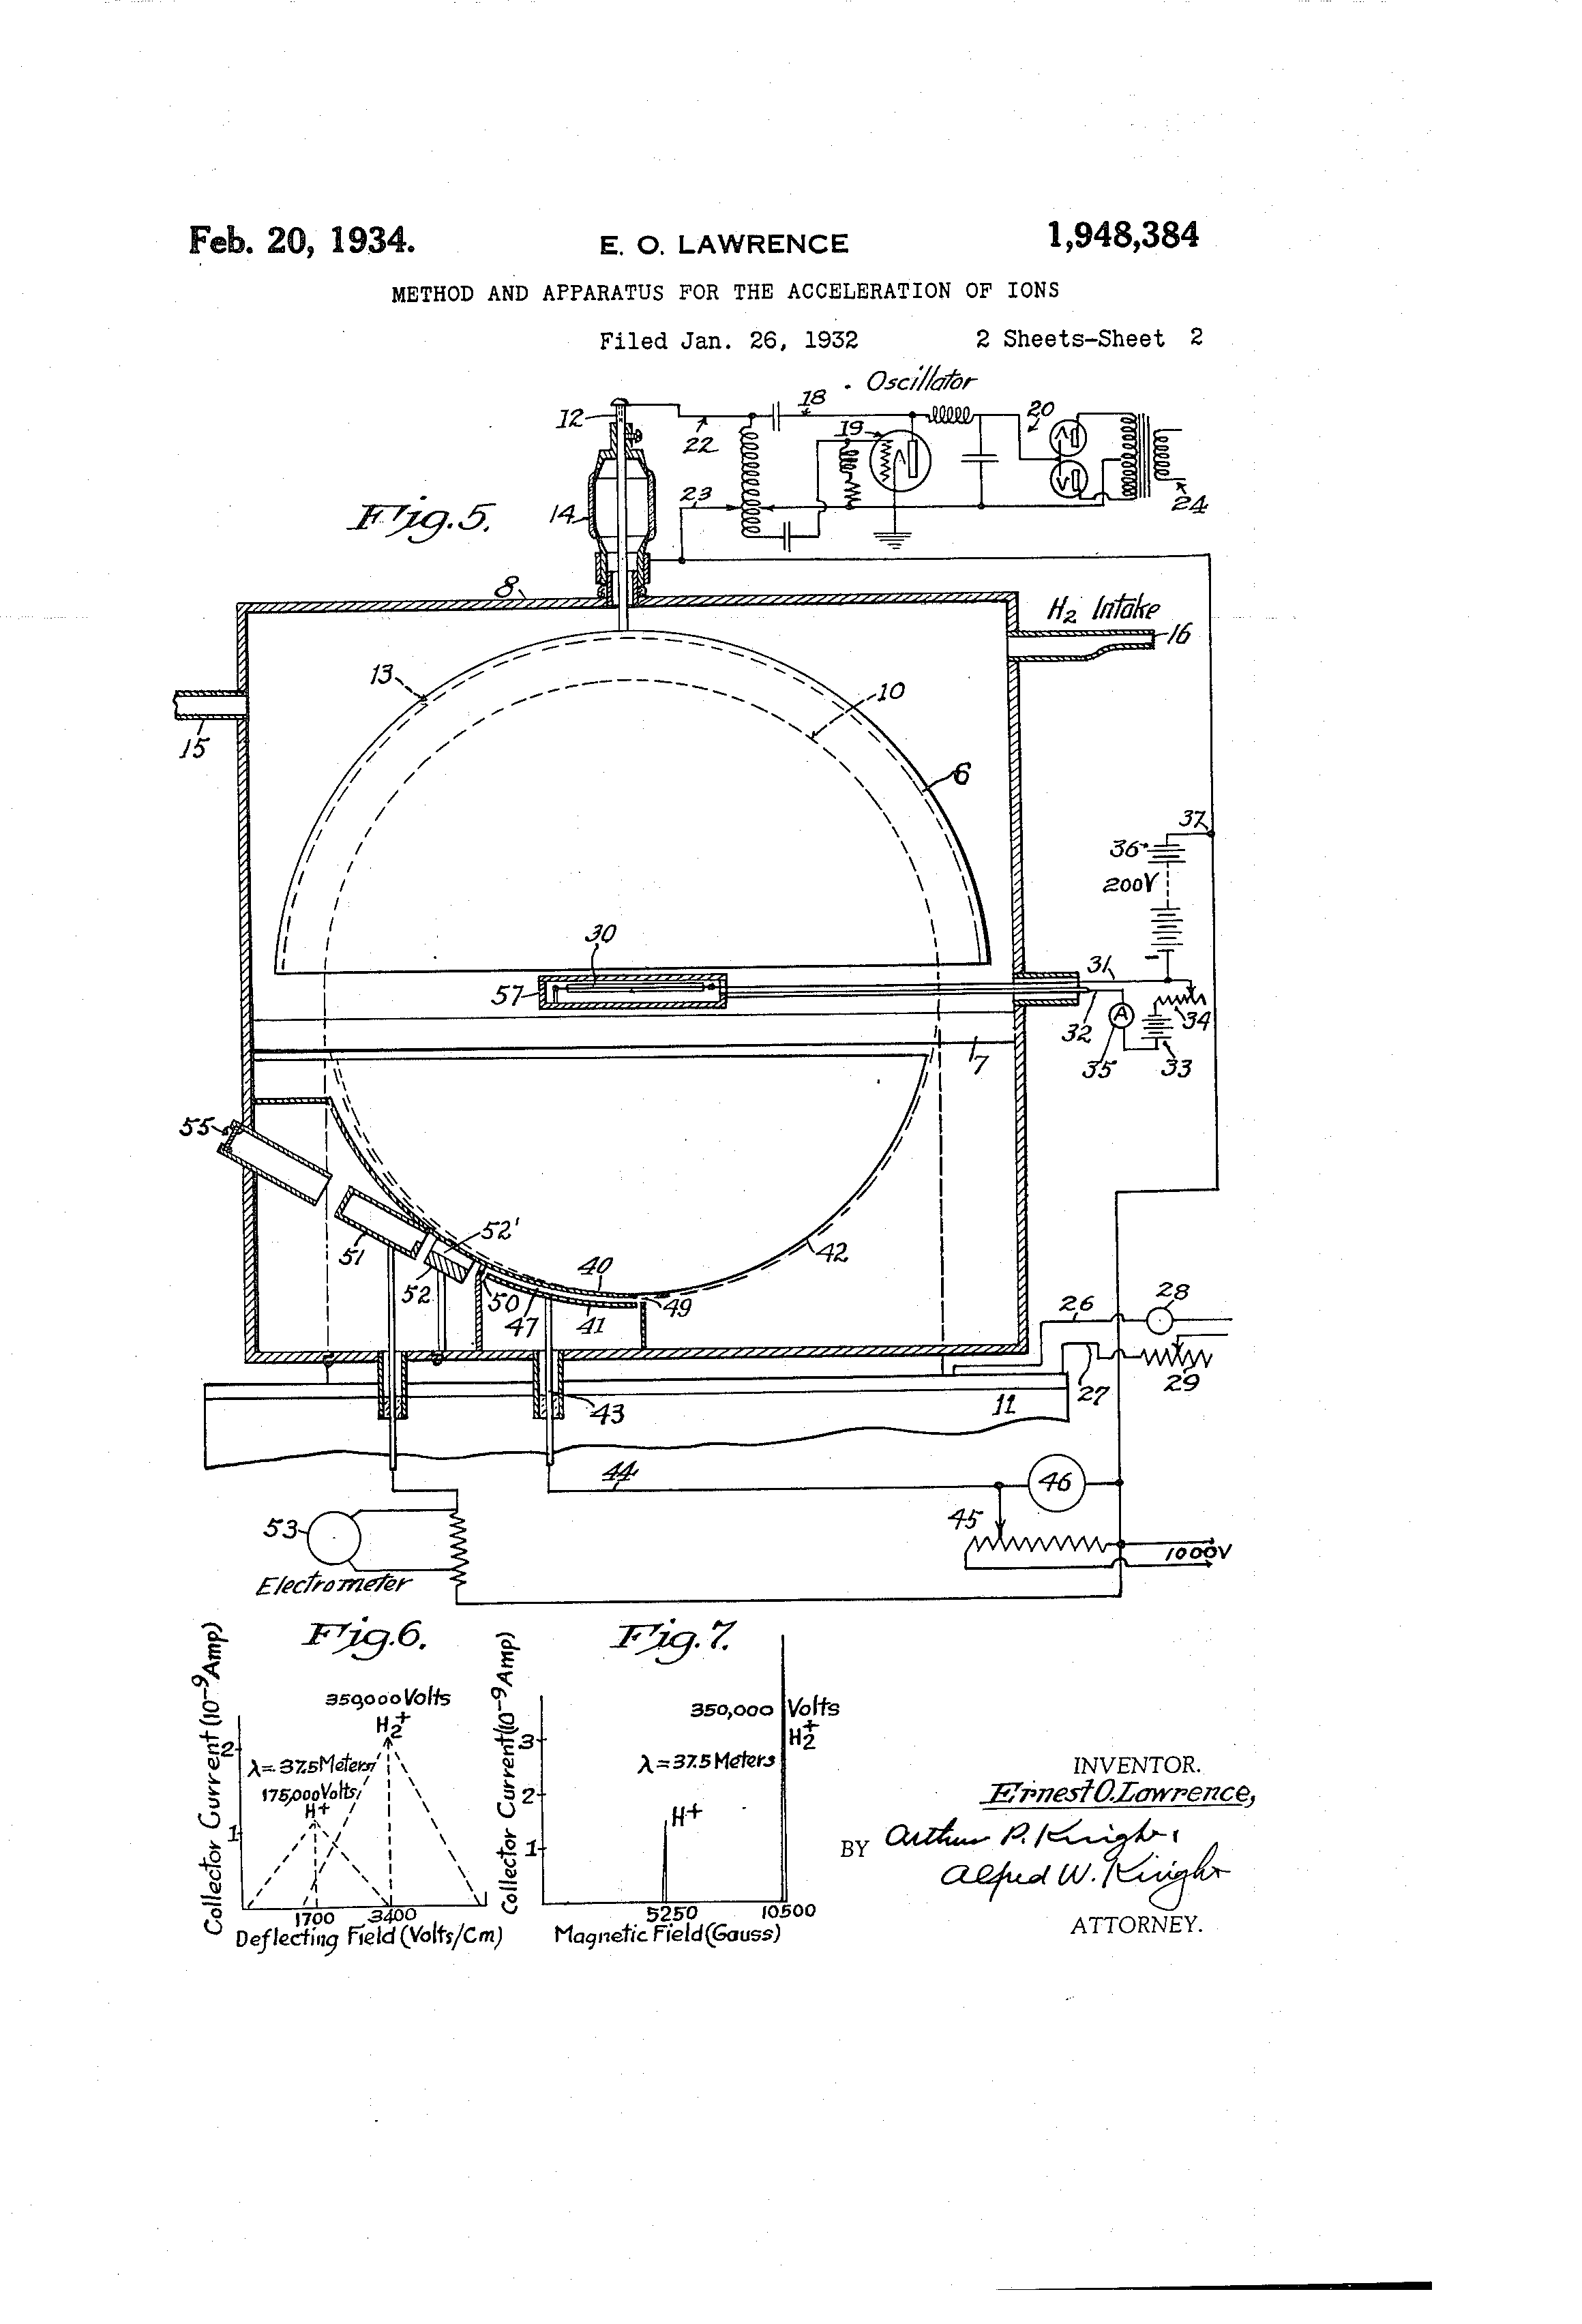
\includegraphics[width=.49\textwidth]{Pictures/cyclo2.png}
  	\caption{\label{fig:cyclo}
                  E. O. Lawrence patent of the cyclotron in the U.S.A.}
  \end{minipage}
\end{figure}

\begin{figure}
 \centering
  \begin{minipage}{\textwidth}
   \centering
    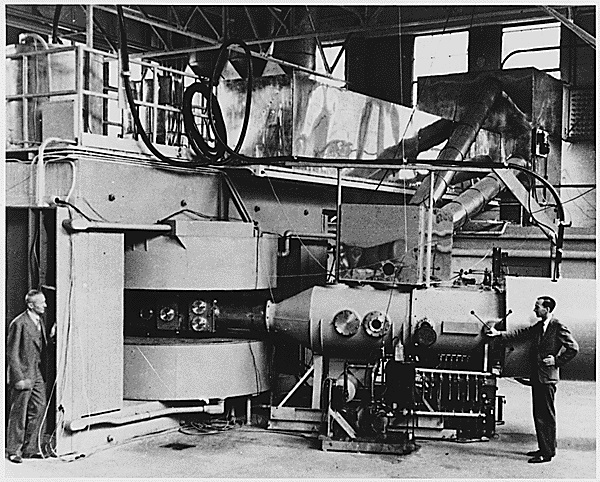
\includegraphics[width=.49\textwidth]{Pictures/cyclo3}
  	\caption{\label{fig:lawrence}
   		E. O. Lawrence next to his 1.5 m in diameter cyclotron
                        at LBNL.
                      \footnotesize{Picture from U.S. Department of Energy}}
  \end{minipage}
\end{figure}

% Betatron
Using yet another of Wider\"oe's ideas, Donald Krest built a machine in 1940
that would keep an almost constant orbit while accelerating the electrons. This
is achieved by increasing the magnetic field over time. Betatrons where widely
used in hospitals as sources of X-rays.
% microtron %nothing relevant to say here
% Synchrotron
In 1944 Vladimir Veksler \cite{veksler} and separately in 1945 Edwin McMillan
\cite{PhysRev.McM} published the principles of phase stability which relates the
synchronicity of the orbiting particles and the electric field of the
time-varying RF. Using this principle Frank Goward and D.E. Barnes built the
first synchrotron by modifying an existing betatron in England
\cite{GOWARD1946}. The second synchrotron accelerator was built by General
Electric Research Laboratory (GERL) and it was here were synchrotron radiation
was first observed. This effect will be further discussed in chapter \ref{c:sr}.


Given the large mass of protons compared to electrons, they become
ultrarelativistic at much higher energies, this posses a difficulty to
synchrotrons: They need to increase the magnetic field as they gain energy. This
technological problem had the effect of proton synchrotrons developing much
latter. Te cosmotron was the first synchrotron to achieve the \SI{}{GeV} regime
\cite{cosmotron}, and the first one to use the beam for external experiments
\cite{cosmotron2}.

After the idea of strong focusing was developed, using focusing-defocusing
quadrupole magnets, it became possible to reach even higher energies. The CERN
Proton Synchrotron started operating in 1959, and it reached energies of 28
GeV.

% colliders
A machine to collide beams, hence greatly improving the energy released, was
first patented by Wider\"{o}e in 1943\cite{birth}. The patent design is shown in
Fig. \ref{fig:wid:collider}. Although some people would
consider that idea to be trivial and obvious \cite{Amaldi}, It was irrelevant at
that time because the repetition rate would have been to low. It was until
storage rings were developed, that colliders became a practical application.
\begin{figure}
 \centering
  \begin{minipage}{\textwidth}
   \centering
    \includegraphics[width=.95\textwidth]{Pictures/collider.jpg}
    \caption{\label{fig:wid:collider}
        Original diagram from the collider patent by Wider\"oe
                       \footnotesize{Picture taken from \protect{\cite{wid:book}}}}
  \end{minipage}
\end{figure}
% ISR
The first circular proton collider consisted on protons accelerated in the
Proton Synchrotron (PS) and then transferred to the newly built Intersecting
Storage Rings (ISR) in 1971. The layout is shown in fig. \ref{fig:isr}. The ISR
had \SI{300}{m} in diameter, The maximum design energy was \SI{28}{GeV}, but the
bunched could be further accelerated in the ISR up to \SI{31.4}{GeV} at the
price of reduced luminosity\cite{isr}. It had eight intersections where the
collisions had place. To achieve its maximum current of \SI{20}{A} it was
required to empty the PS several times into each of the two rings.

\begin{figure}
 \centering
  \begin{minipage}{\textwidth}
   \centering
    \includegraphics[width=.95\textwidth]{Pictures/isr.jpg}
    \caption{\label{fig:isr}
        Layout of the ISR
                       \footnotesize{taken from \protect{\cite{isr}}}}

  \end{minipage}
\end{figure}

% light sources
In 1973 at the Stanford Positron Electron Accelerating Ring (SPEAR), researchers
realized that the SR emitted by the beam was too high to allow it to go to
waste, hence creating the Stanford Synchrotron Radiation Laboratory
(SSRL). Although the goal of SSRL was to take advantage of the
`wasted' energy emitted as SR, eventually SPEAR became solely dedicated to
SSRL. Nowadays there are several accelerators around the world dedicated only
to emit SR, these are known as light sources.

Accelerators around the world kept growing in numbers, size, energy reach, and
luminosity over the following years. An important technological development in
the decade of 1970 was the use of superconducting materials to greatly improve
the efficiency of RF cavities and bending magnets.

In 1983 Fermi National
Accelerator Laboratory (FNAL) replaced its main ring to an proton-antiproton
accelerator and collider with center of mass (CoM) collision energy of
\SI{1.8}{TeV}. It was called the Tevatron, the first accelerator reaching
energies superior to \SI{1}{TeV}. It remained the highest energy collider until
the construction of LHC which is further discussed in section \ref{lhc}.


\section{Working Principles}
Accelerators rely solely in the manipulation of electromagnetic fields 
\section{LHC}
\label{lhc}
%----------------------------------------------------------------------------------------
The Large Hadron Collider (LHC) at CERN is a wonder of engineering and
technology. It lies inside a 26.7 Km circular tunnel and 100 meters under the
ground. Its construction took over 15 years, involved engineers from all over
the world and costed over 6.5 billion CHF. Inside the tunnel there are two
counter-rotating hadron beams accelerated to energies up to 7 TeV each. This
beams are then forced to collide inside four huge detectors that measures the
products of the collision\citep{LHCMT}.
\subsection{Characteristics}
The 26,659 m tunnel used by the LHC was inherited from the LEP, when it was shut
down. The basic layout consists of eight long straight sections and eight
bending arcs\citep{keil}. In order to keep the 7 TeV proton beams in such a
small orbit it was necessary to use 1,232 magnets with a 8.3 T field that extend
to a length of 14.3 m each\citep{DR}. To achieve this, powerful magnetic field
superconducting magnets were to be used. Because of commercial availability NbTi
superconductors were used, this material needs to be cooled down below 4.2 K to
reach the superconducting state.  The solution was, and still is, to keep the
magnets submerged in superfluid Helium below 2 K\citep{keil}.  The basic layout
is shown in Figure \ref{Schem}, where Beam 1 is shown in blue and circulates
clockwise; and in red Beam 2 which rotates counterclockwise. There are four
intersections, one in each major experiment: ATLAS, CMS, LHC-b, and ALICE. The
first two, ATLAS and CMS, are high luminosity experiments and are located
diametrically opposite to each other, while LHC-b is an devoted to quark b
experiments, and ALICE stands for A Large Ion Collider Experiment, which is
self-explanatory and work with full stripped Pb ions. The LHC consist of 8 arcs
and 8 straight section and it is divided in octants, that start at the center of
on arc and end at the center of the next one\citep{DR}.
\begin{figure}
	\centering
  \begin{minipage}{\textwidth}
  	\centering
   	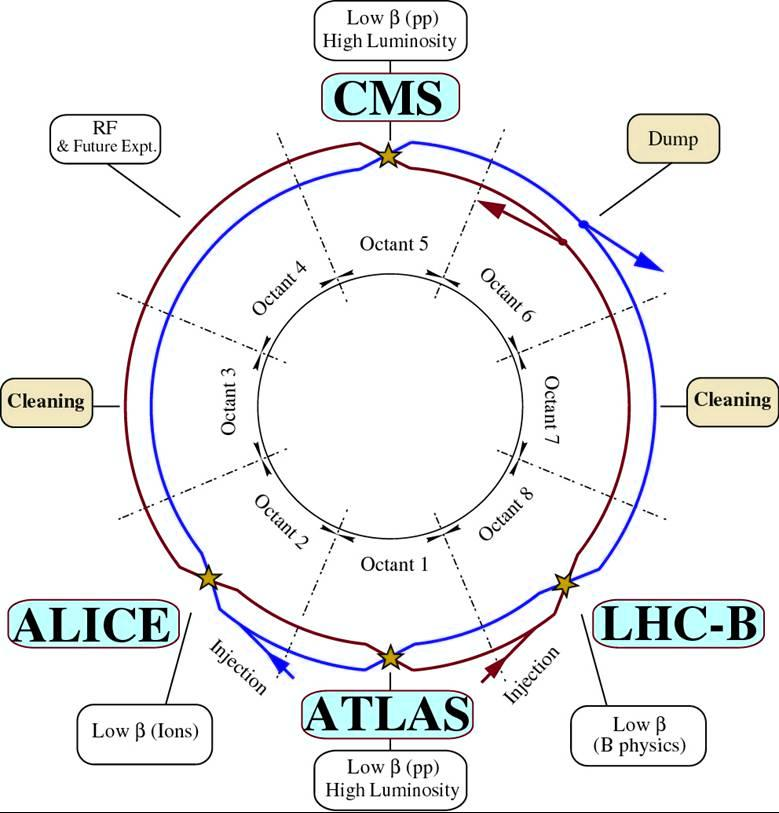
\includegraphics[width=3.5in]{Pictures/imagen.jpg}
  		\caption{\label{Schem}
   			General schematic for the LHC}
   			\footnotesize{Picture courtesy of CERN.}
   \end{minipage}
\end{figure}
The main parameters when working at its maximum energy are listed in Table \ref{table:LHCparam}. 
\begin{table}%[ht]
%\centering % used for centering table
\caption{Main parameters for proton-proton collisions} % title of Table
\begin{minipage}{\textwidth}
\renewcommand{\thefootnote}{\thempfootnote}

%\footnote{This table was taken from "the LHC vacuum system", p. 292 \citep{vacuum}. }
\begin{tabular}{l c}% centered columns (4 columns)
\hline
Energy \hspace{8.5cm} & 7 TeV \\ % inserting body of the table
Dipole Field & 8.33 T \\
coild aperture & 56 mm \\
Luminosity &10\textsuperscript{34} s\textsuperscript{$-$1} cm\textsuperscript{$-$2} \\
Injection energy & 450 GeV \\
Circulating current/beam & 0.56 A\\
Bunch spacing & 25 ns \\
Particles/bunch & 1.1$\times$10\textsuperscript{11} \\
Stored beam energy & 350 MJ \\
Normalised trasverse emittance & 3.75 $\mu$m \\
RMS bunch length & 0.075 m \\
Beam lifetime & 22 h \\
Luminosity lifetime & 10 h \\
Energy loss/turn & 6.7 keV \\
Critical photon energy & 45 eV \\
Linear photon flux & 1$\times$10\textsuperscript{17} m\textsuperscript{$-$1}s\textsuperscript{$-$1} \\
Total radiated power/beam & 3.8 kW \\ [1ex] % [1ex] adds vertical space
\hline
\end{tabular}
\end{minipage}
\begin{minipage}{\textwidth}
\begin{footnotesize}
* This table was taken from "the LHC vacuum system", p. 292 \citep{vacuum}.
\end{footnotesize}
\end{minipage}
\label{table:LHCparam} % is used to refer this table in the text
\end{table}

\subsubsection{Arc Cells}
The arcs consist of 23 regular arc cells. These are made out of two 53.45 m long half cells each of which consist of one cold mass with a length of 5.355m (6.63 mlong cryostat) short straight section (SSS) assembly and three 14.3 m long dipole magnets. The optics of Beam 1 and Beam 2 are coupled by electrical connections of the main magnets. There is also a dispersion suppressor at every transition between arcs and straight sections. The arc cells emulate a FODO lattice\citep{DR}.
\subsection{Optics}
The LHC optics design allows an optics matching with fixed and equal phase advances over the insertion regions for both beams that does not perturb the optics in the rest of the machine. The total number of particle trajectory oscillations during one revolution in the storage ring of the machine is adjusted by the optics of the arc cell. The flexibility of the phase advance over the insertions provides a measure for the flexibility of the total LHC optics and tell us how much liberty we have to change the phase advance between the main experimental insertions\cite{DR}.

\subsection{LHC Beam Pipe}
Because of the high beam intensities given by luminosities such as the one shown in Table \ref{table:LHCparam}, the LHC cannot work the same way as the Tevatron, which uses a single vacuum chamber and one set of magnets for both beams, the LHC requieres a vacuum chamber and set of magnets for each beam, and the beams only share the regions where the collisions take place and are around 130 m long\citep{DR}.
On one hand we have the price of the magnets and on the other hand we have the problem that there is not enough space in the LEP tunnel for two sets of magnets; as a result the LHC was built with twin bore magnets constructed of two sets of coils and beam channels within the same mechanical structure and cryostat\citep{DR}.

\textcolor{black}{90\% of the LHC surface should be maintained below 20 K and is made of copper cladded stainless steel in order to reduce ohmic resistence. The rest can stay at room temperature and is made of thick copper beam pipe \citep{DR}.}


\label{screen}
Another important feature of the beam pipe is the beam screen, this is a cooled screen intended to intercept SR at temperatures higher than 1.9 K and electrons due to electron clouds in order to prevent the magnets from heating. Figure \ref{fig:screen} shows the conceptual design of the LHC beam screen\citep{DR}\citep{vacuum}. 
\textcolor{black}{
The manufacturing process starts by co-laminating a specially developed low permeability 1mm thick
austenitic stainless steel strip with a 75 $\mu$m copper sheet and rolling a saw-tooth structure which  will intercept photons at normal incidence, thereby reducing the amount of reflected photons. The pumping slots are punched into this composite strip, which is then rolled into its final shape and closed by a longitudinal
weld\citep{vacuum}.
}
\begin{figure}
	\centering
  \begin{minipage}{\textwidth}
  	\centering
   	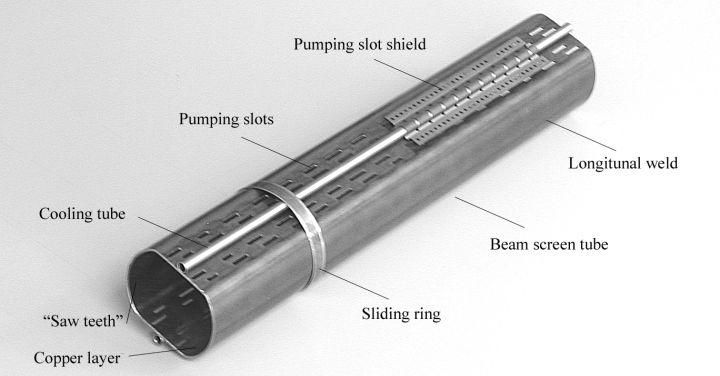
\includegraphics[width=3.5in]{Pictures/screen.png}
  		\caption{\label{fig:screen}
   			LHC Beam Screen}
   			\footnotesize{Picture courtesy of CERN.}
   \end{minipage}
\end{figure}

\subsection{Cryogenics}
\label{cryo}
The LHC uses cryomodules that consume liquid helium and expel evaporated helium. Each module looses 150 W statically in addition to the dynamic losses, that span from 100 W to 800 W.
For operation at nominal field the pressure inside the helium tank has to be carefully controlled to avoid frequency variations of the cavity\citep{DR}.
\subsection{Synchrotron Radiation}
The LHC is the first proton collider for which SR is a problem. At its highest energies SR gives rise to an important heat load to the beam screen\citep{DR}, mentioned in \ref{screen}. As shown in Table \ref{table:LHCSR} each beam produce an average of 6.8 $\times$ 10\textsuperscript{16} photons per metre per second in the arcs, which corresponds to 3886 W. So the SR power per metre per bend per beam is 220 mW/m. 

\begin{table}%[ht]
\caption{SR Parameters} % title of Table
%\centering % used for centering table
\begin{minipage}{\textwidth}
\begin{tabular}{l c c}% centered columns (4 columns)
\hline
\hline %inserts double horizontal lines
Parameter & 450 Mev & 7 TeV \\[0.5ex]% inserts table heading
\hline % inserts single horizontal line
Total power/beam & 0.066 W & 3886 W \\ % inserting body of the table
Energy loss per turn & 0.11 eV & 6.7 keV \\
average photon flux per metre and second & 0.4 $\times$ 10\textsuperscript{16} & 6.8 $\times$ 10\textsuperscript{16} \\
Photon critical energy & 0.01 eV & 43.13 eV \\
Longit. emittance damping time & 5.5 yr & 12.9 h \\
Trans. emittance damping time & 11 yr & 26 h \\ [1ex] % [1ex] adds vertical space
\hline %inserts single line
\end{tabular}
\end{minipage}
\begin{minipage}{\textwidth}
\begin{footnotesize}
* This table was taken from the "LHC Design Report", p. 108 \citep{DR}.
\end{footnotesize}
\end{minipage}
\label{table:LHCSR} % is used to refer this table in the text
\end{table}

%----------------------------------------------------------------------------------------


\subsection{Electron Cloud Due to Beam Induced SR}

When high energy SR photons strike a surface, they are able to set loose
electrons out of the surface by ionizing it. This electrons are then attracted
by the protons in the beam, they move, hitting the wall extracting even more
electrons out of the wall, that will follow the next bunch of protons, this
process leads to a fast building electron cloud, which is a very undesirable
effect. The effects of electron clouds have been studied at CERN since
1997\cite{rumolo2011electron}.


%\subsection{Sawtooth Pattern}
%----------------------------------------------------------------------------------------

\subsection{HL-LHC}
\section{FCC}
\subsection{HE-LHC}
\subsection{FCC-hh}
\subsection{FCC-ee}
\subsection{FCC-he}
